\chapter{BERTopic}
L'avvento dei moderni \emph{LLM} ha portato ad un'evoluzione del \textbf{NLP} (Natural Language Processing) con la conseguente nascita di nuovi framework e tecniche per le analisi più disparate.
Il \emph{topic modeling} non è esente da questo fenomeno, in particolare i modelli basati su \textbf{transformers} (cioè modelli che convertono testo in embeddings dipendenti dal contesto) si sono rilevati particolarmente efficaci.% nell'\emph{nlp}.
\textbf{Modelli preaddestrati} sono molto utilizzati perché permettono di creare rappresentazioni \textbf{accurate} e \textbf{rappresentative} di testi, potendo fare affidamento su dataset di training molto grandi e molto diversificati.
In questo contesto BERTopic è un \textit{framework} al passo con il corrente stato dell'arte, che offre alcuni vantaggi rispetto a tecniche antecedenti, fra cui permette di catturare il \textbf{significato semantico} dei documenti (riconosce ad esempio i sinonimi). Per dataset eterogenei e rumorosi come gli annunci di lavoro, questa capacità di individuare strutture semantiche latenti rende BERTopic una scelta particolarmente vantaggiosa rispetto ai modelli tradizionali. Inoltre in BERTopic specificare il il numero di classi è \textbf{opzionale}.
Inoltre BERTopic è composto da più \textit{submodules} con funzioni diverse, il che permette un'alta personalizzazione.

\section{Funzionalità}
All'interno di Bert Topic è possibile distinguere alcune funzionalità particolarmente utili per questo progetto:
\begin{enumerate}
\item Embedding
\item Dimensionality Reduction
\item Clustering
\item Tokenizer
\item c-TF-IDF
\end{enumerate}

BERTopic permette l'utilizzo di algoritmi diversi per ogni funzionalità, per personalizzare il proprio \emph{topic model}, ad esempio il clustering può essere effettuato da \emph{HDBSCAN} o da \emph{k-Means}.
Illustreremo ora tutti i moduli da noi usati, vedremo nello specifico la loro funzione e come la loro alterazione modifica il risultato finale.
\subsection{Embedding}
Il primo modulo è l'\textbf{embedder}, il cui compito è quello di trasformare i documenti in rappresentazioni numeriche.
i modelli principali consigliati nella documentazione\footnote{\url{https://maartengr.github.io/BERTopic/getting_started/embeddings/embeddings.html}} sono i \textbf{sentence transformers} (SBERT).
Ci sono molti modelli SBERT pre-addestrati tra cui scegliere, la documentazione ufficiale nei suoi esempi usa spesso all-MiniLM-L6-v2 un modello estremamente leggero e veloce, però non sufficientemente preciso nel catturare sfumature semantiche complesse o relazioni a lungo raggio.
paraphrase-MiniLM-L12-v2 e paraphrase-mpnet-base-v2, sono più accurati, ma più specializzati nel catturare relazioni di parafrasi, fra testi molto simili, sono inoltre inadatti a testi particolarmente lunghi come gli annunci di lavoro.
\textbf{all-mpnet-base-v2}, invece, ha una alta \textbf{precisione semantica}, e si comporta bene con documenti di lunghezza \textbf{medio-lunga}.
Ha però un limite di lunghezza di \textbf{512 token}, con token in questo contesto ci riferiamo all' unità base che usano i modelli sentence transformers, i token sono composti da una parola o da una frazione di essa.
Ecco alcune informazioni sulla lunghezza del nostro dataset (dopo la pulizia):
\begin{figure}[H]
\centering
\scriptsize
\begin{tabular}{lccc}
\hline
 & n chars & n words & n tokens mpnet \\
\hline
count & 5357.00 & 5357.00 & 5357.00 \\
mean & 3315.48 & 457.92 & 594.54 \\
std & 1591.28 & 219.01 & 283.37 \\
min & 91.00 & 14.00 & 23.00 \\
50\% & 3087.00 & 427.00 & 554.00 \\
75\% & 4060.00 & 562.00 & 729.00 \\
90\% & 5213.40 & 717.00 & 934.00 \\
95\% & 6188.20 & 846.20 & 1103.40 \\
99\% & 8797.52 & 1203.44 & 1562.72 \\
max & 19470.00 & 2739.00 & 3753.00 \\
\hline
\multicolumn{4}{l}{Testi che superano i 512 token: 3075 (57.40\%)} \\
\multicolumn{4}{l}{Totale annunci: 5357} \\
\hline
\end{tabular}
\caption{Statistiche globali del dataset (totale annunci: 5357).}
\label{fig:dataset-stats}
\end{figure}
\noindent Quando SBERT riceve un input troppo lungo, lo \textbf{tronca} questo significa che applicando l'embedder così come è verrebbe tagliata una porzione molto grande del dataset.

\noindent Le prime opzioni che abbiamo considerato sono:
\begin{enumerate}
    \item Affidarsi ad un modello con un limite di dimensione input più alto (ad esempio \textbf{all-roberta-long-v1})
    \item Frammentare le descrizioni e fare il topic modeling in segmenti di quest ultime.
\end{enumerate}
Il vantaggio della prima opzione è che i modelli \textit{long-context}, mantengono attenzione tra termini distanti, permettendo di cogliere relazioni semantiche a lungo raggio, cosa impossibile se si divide il testo in \textit{chunk}.
Non è però una caratteristica che abbiamo ritenuto significativa, data la natura del nostro \textit{dataset}, infatti i nostri paragrafi hanno natura scollegata, uno potrebbe parlare di competenze e un altro di mansioni, la coerenza globale è più importante in testi di natura \textbf{discorsiva}.
Inoltre se la lunghezza del testo è grande è probabile che contenga più temi, un unico embedding rischia di mescolare \textbf{sezioni semanticamente diverse}, ottenendo topic più grossolani.
La seconda opzione invece oltre che generare topic più \textbf{puliti} e \textbf{interpretabili}, consente di aumentare molto il numero di documenti in input, questo è un vantaggio per dataset esegui come il nostro.
Però anche questo caso presenta delle criticità: non avremmo i topic relativi agli annunci, questi ultimi andrebbero aggregati a posteriori per ottenere una \textbf{distribuzione di topic per documento}. In più in questo modo, gli annunci più lunghi hanno \textbf{più peso}, semplicemente perché hanno più paragrafi, la situazione si complica ulteriormente se i documenti contengono paragrafi simili, questo creerebbe dei \textbf{cluster} artefatti e quindi topic che non rispecchiano la natura del dataset. Un altro problema è che con questo metodo il modello è completamente ignaro della struttura globale dell'annuncio.
Questo approccio è più attuabile per risolvere un problema di \textbf{classificazione}, non per il \textit{topic modeling}.\medskip

\noindent La soluzione che abbiamo scelto è dunque quella di \textit{mean-max-pooling}.
\subsubsection{Mean-max pooling}

\noindent Con questa tecnica si ottiene un embedding per ogni annuncio partendo dagli embedding dei paragrafi, seguendo i passaggi seguenti:
\begin{enumerate}
    \item calcolare gli embedding di ciascun paragrafo;
    \item normalizzare ogni embedding;
    \item calcolare media aritmetica e massimo elemento per elemento;
    \item concatenare i due vettori risultanti;
    \item normalizzare nuovamente il vettore concatenato.
\end{enumerate}

In questo modo si ottiene un embedding unico di dimensione doppia rispetto l'output dell'embedder che cattura sia il \textbf{significato generale} dell'annuncio, sia le \textbf{feature salienti} dei singoli paragrafi: queste due componenti producono vettori più \textbf{discriminativi} e quindi più facilmente separabili nello spazio semantico.

Per attuare questo approccio serve inoltre una strategia di segmentazione degli annunci che soddisfi al contempo \textbf{coerenza semantica} e criteri di lunghezza: il segmento non può essere troppo corto, altrimenti SBERT non ha il contesto per estrarre topic, e non può ovviamente superare la lunghezza massima consentita. Approfondiamo questo aspetto nel capitolo \textbf{Pre-processing}.
\subsection{Dimensionality Reduction}
I vettori generati dall'embedder hanno dimensione 768, ciò potrebbe rendere difficile il \emph{clustering} per questo è importante introdurre nella pipeline un algoritmo di riduzione della dimensione.
L'idea di questi algoritmi è quella di ridurre la dimensione di un insieme di vettori preservandone la \textbf{struttura topologica locale}.
Di default BERTopic usa \textbf{UMAP}\footnote{\url{https://maartengr.github.io/BERTopic/getting_started/dim_reduction/dim_reduction.html}} per questo compito poiché \emph{preserva sia la struttura locale, che quella globale degli spazi ad alte dimensioni}.
UMAP lavora costruendo un \textit{grafo fuzzy locale}: ogni punto viene connesso ai suoi n\_neighbors più vicini e la connessione è pesata in base alla distanza. Questo grafo rappresenta la topologia locale dello spazio originale.
UMAP cerca poi una rappresentazione a bassa dimensione che minimizzi la differenza tra il grafo originale e il grafo proiettato.

L'obiettivo è mantenere la densità e la vicinanza dei punti simili, consentendo allo stesso tempo di contrarre regioni sparse.
Questo bilanciamento consente di preservare la struttura locale pur comprimendo lo spazio globale.
Vediamo più nel dettaglio questi punti:
\subsubsection{fuzzy simplicial complex}
Per costruire il grafo iniziale ad alta dimensionalità, \textbf{UMAP} crea una struttura chiamata \textit{fuzzy simplicial complex}. In pratica, si tratta di una rappresentazione di un grafo pesato, in cui i pesi degli archi rappresentano la \textbf{probabilità che due punti siano connessi}.

Per determinare la connessione tra due punti, UMAP\footnote{\url{https://pair-code.github.io/understanding-umap/}} estende un \textbf{raggio locale} a partire da ciascun punto e collega i punti quando i rispettivi raggi si sovrappongono. La scelta di questo raggio è cruciale:
Se è troppo piccolo, il risultato sarà un insieme di \textbf{piccoli cluster isolati};
se è troppo grande, tutti i punti finiranno per essere \textbf{collegati tra loro}, perdendo così la struttura locale.

UMAP risolve questo problema scegliendo un raggio locale \textbf{adattivo}, basato sulla distanza rispetto al $k$-esimo vicino più prossimo di ciascun punto. Successivamente, il grafo viene reso ``sfumato'' (\textit{fuzzy}) diminuendo la probabilità di connessione man mano che la distanza aumenta.

Infine, imponendo che ogni punto sia connesso almeno al proprio vicino più prossimo, UMAP garantisce un equilibrio tra la \textbf{preservazione della struttura locale} e la \textbf{coerenza della struttura globale}.
\begin{figure}[H]
\centering
\includegraphics[width=0.75\textwidth]{img/BERTopic/umap/UMAP\_projection.png}
\caption{Proiezione UMAP nel piano bidimensionale. Dopo l'intersezione con il primo \emph{neighbour}, il cerchio diventa \emph{sfumato}, riducendo il peso della connessione.\protect\footnotemark}
\label{fig:umap-projection}
\end{figure}
\footnotetext{\url{https://pair-code.github.io/understanding-umap/}}
\subsubsection{Parametri}
I due parametri più importanti di UMAP sono \texttt{n\_neighbors} e \texttt{min\_dist}, poiché regolano l'equilibrio tra struttura \textit{locale} e \textit{globale} nella proiezione finale.\footnote{\url{https://pair-code.github.io/understanding-umap/}}

\paragraph{\texttt{n\_neighbors}.} Determina il numero di vicini utilizzato per costruire il grafo fuzzy iniziale. Valori bassi enfatizzano le relazioni locali, isolando micro-strutture anche molto sottili; valori alti favoriscono invece la coerenza complessiva, preservando maggiormente la geometria globale dell'insieme di punti.

Per visualizzare l'effetto di \texttt{n\_neighbors} consideriamo la proiezione bidimensionale di un modello 3D campionato con 50\,000 punti. Le immagini mostrano come la struttura globale emerga gradualmente all'aumentare del numero di vicini, mentre i dettagli fini sono preservati soltanto per valori più bassi.

\begin{figure}[H]
\centering
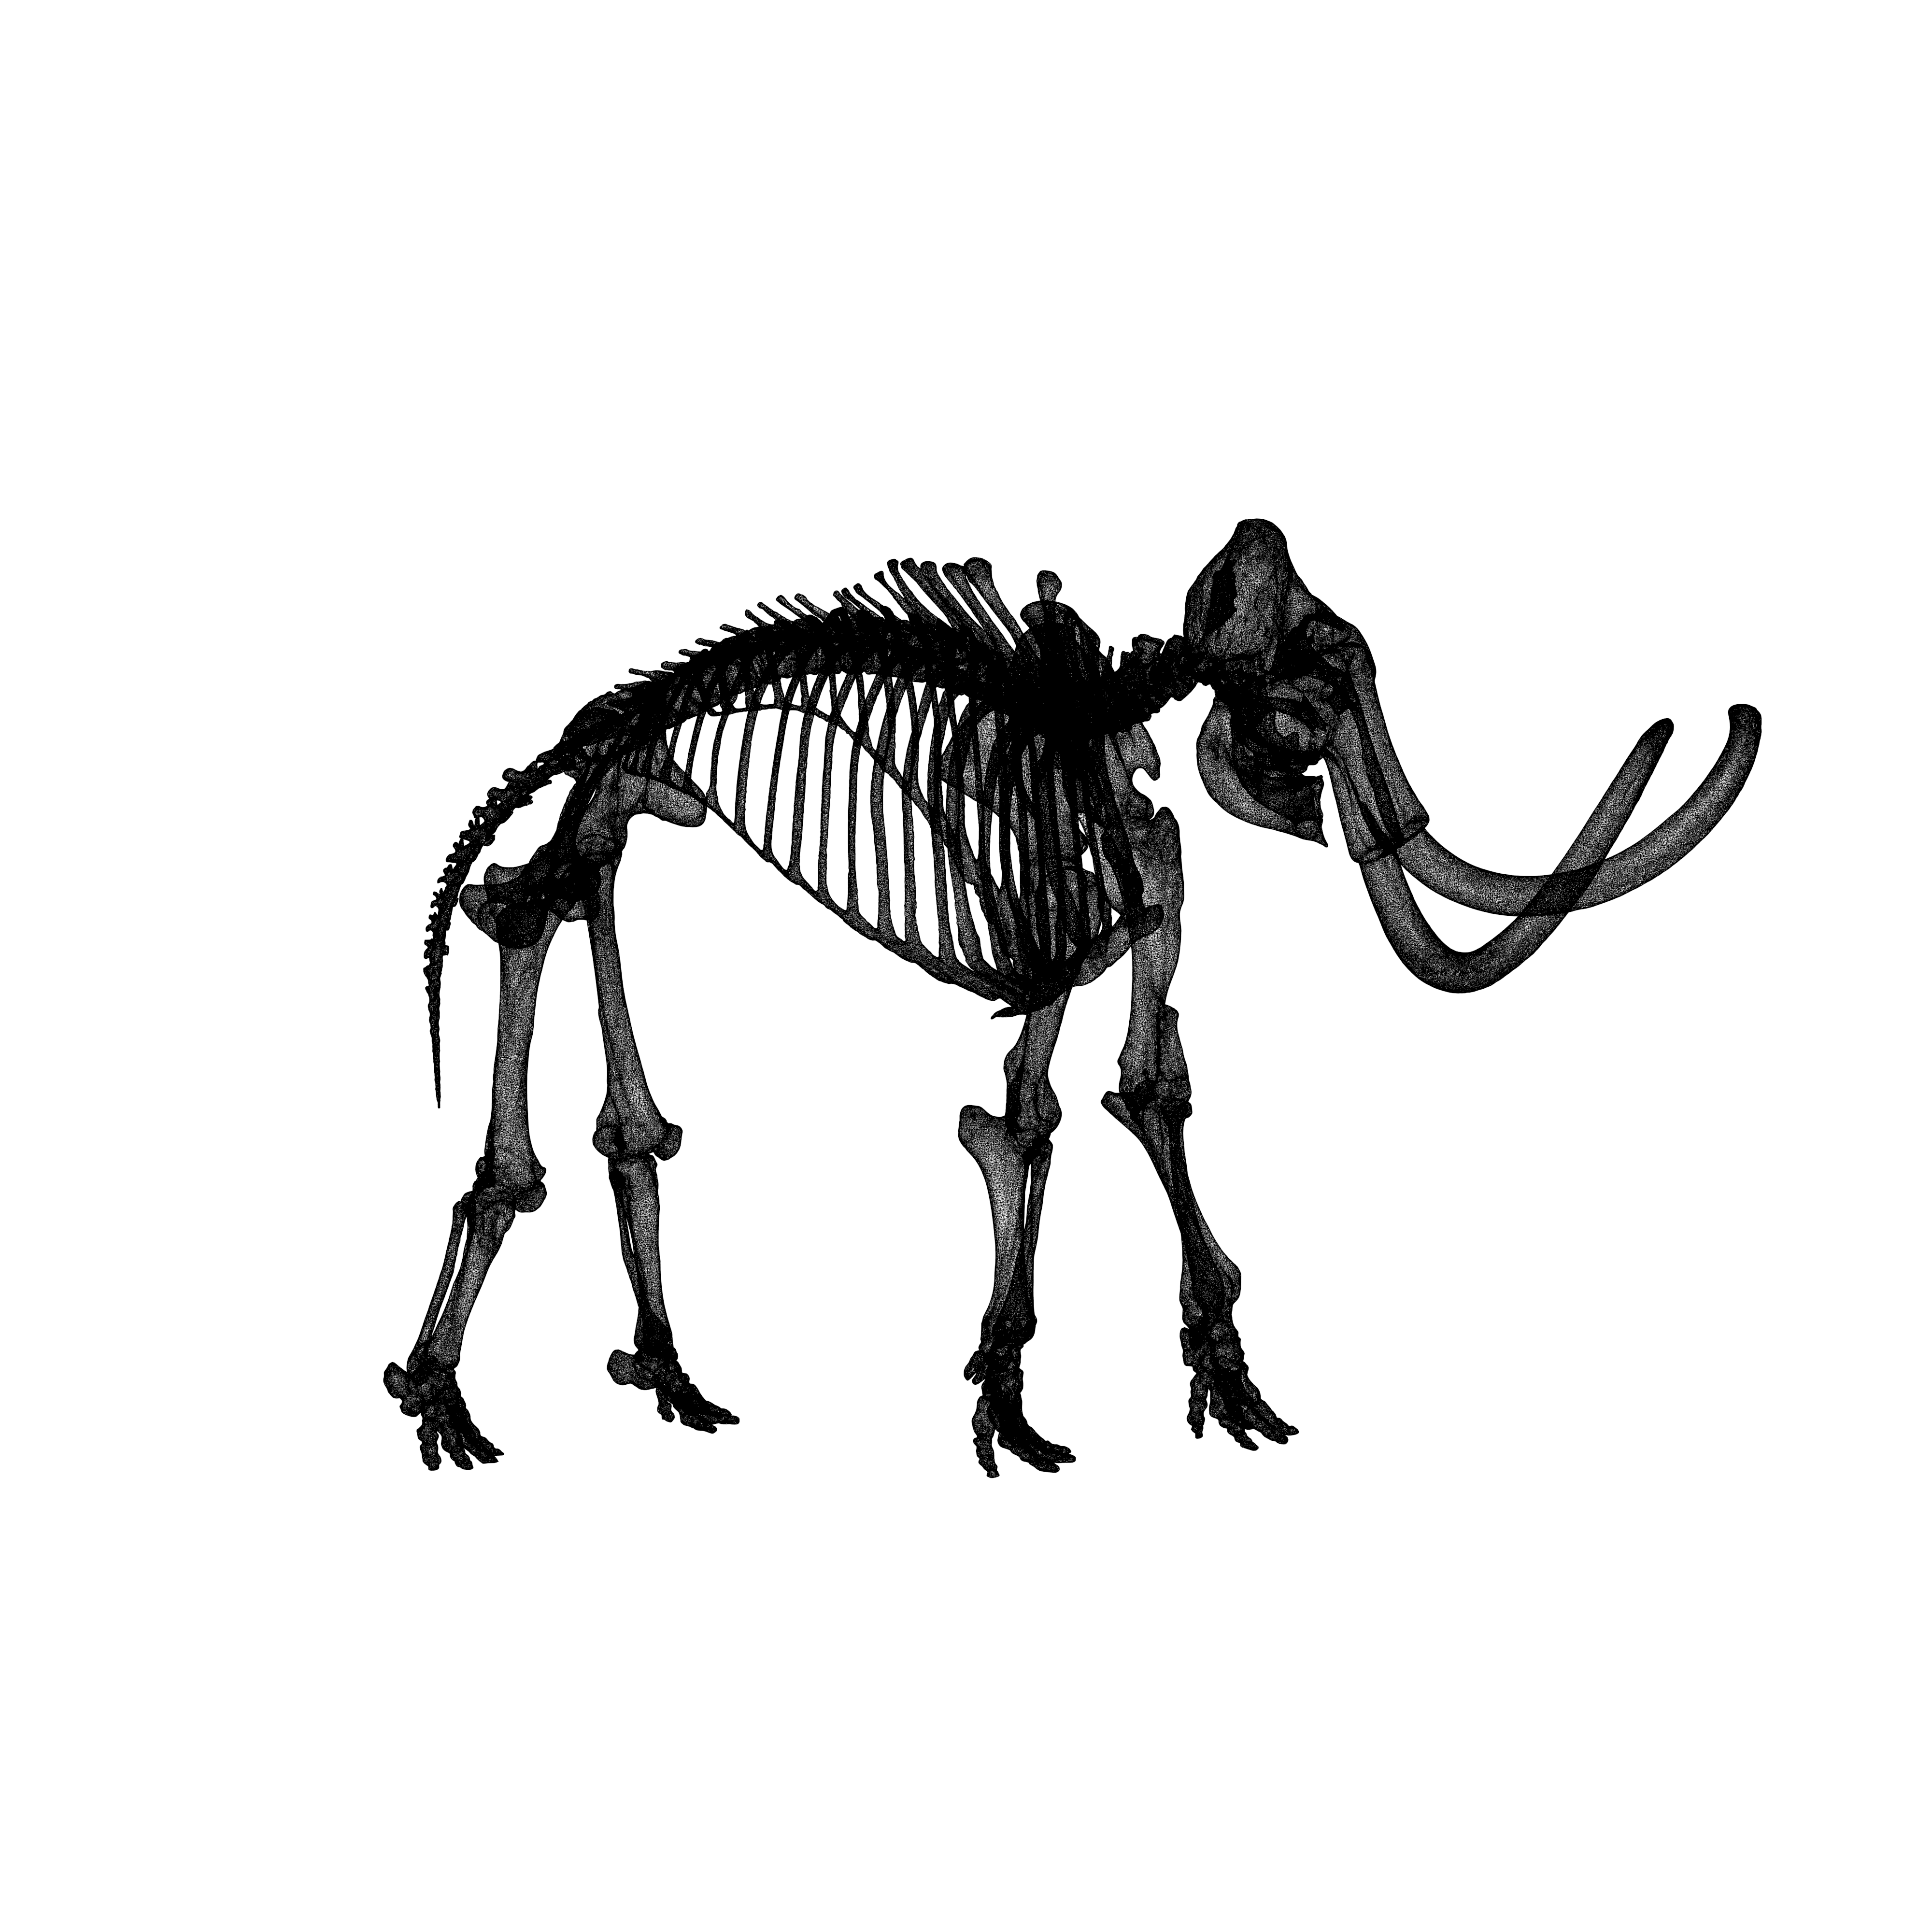
\includegraphics[width=0.5\textwidth]{BERTopic/umap/mammoth_render.png}

\begin{subfigure}{0.32\textwidth}
    \centering
    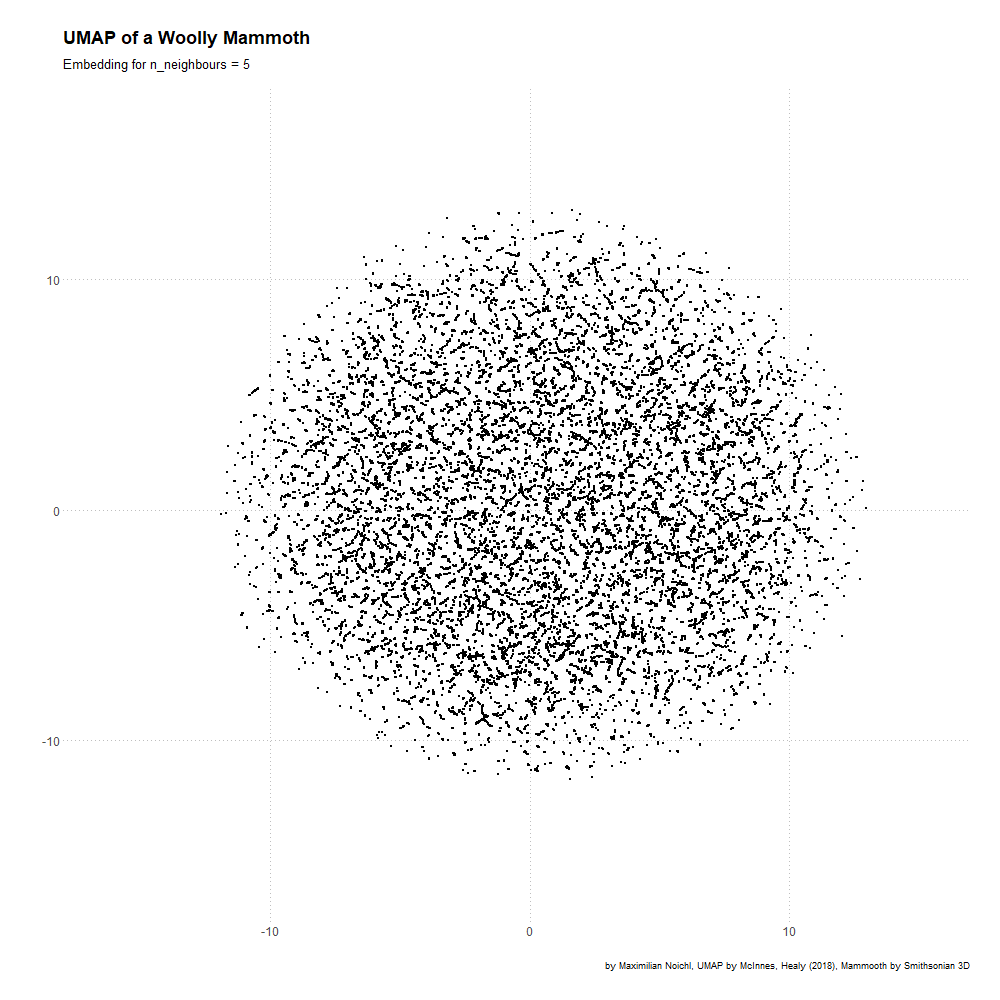
\includegraphics[width=\textwidth]{BERTopic/umap/n_neighbours5.png}
    \caption{$n\_neighbors = 5$}
\end{subfigure}\hfill
\begin{subfigure}{0.32\textwidth}
    \centering
    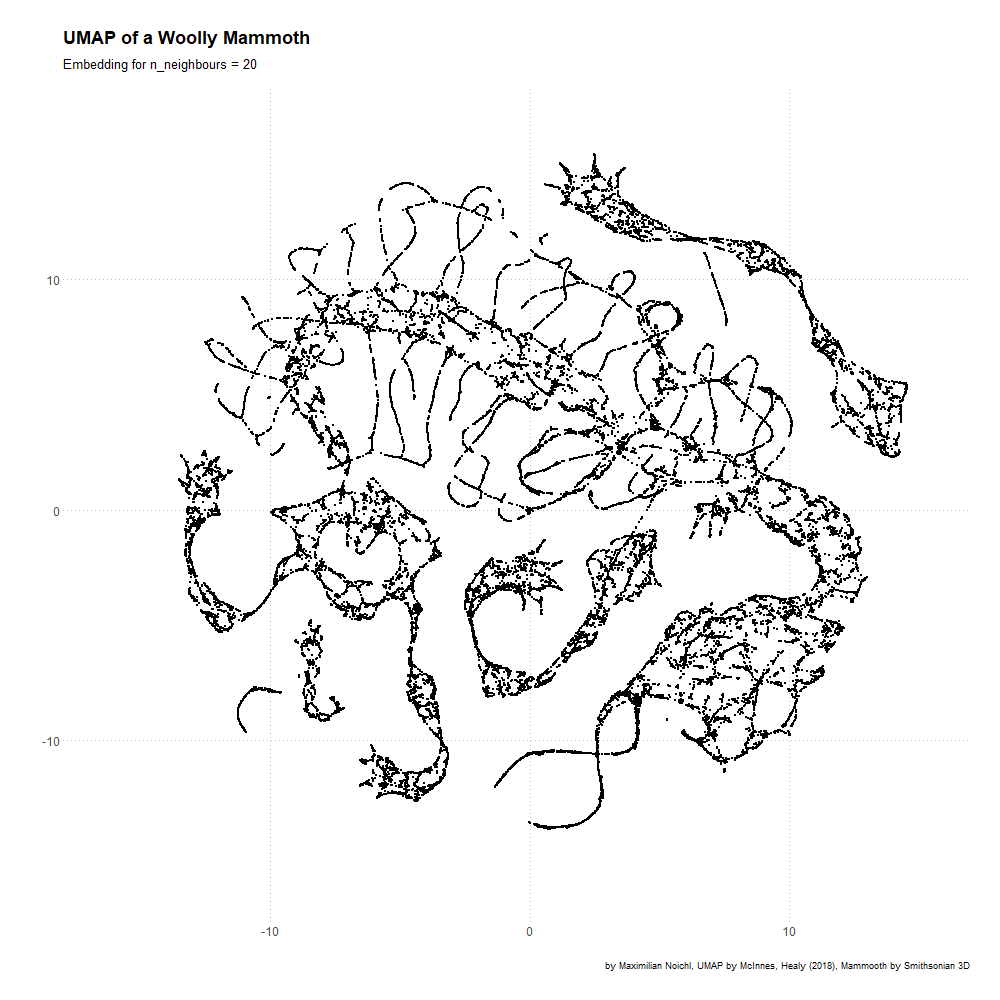
\includegraphics[width=\textwidth]{BERTopic/umap/n_neighbours20.png}
    \caption{$n\_neighbors = 20$}
\end{subfigure}\hfill
\begin{subfigure}{0.32\textwidth}
    \centering
    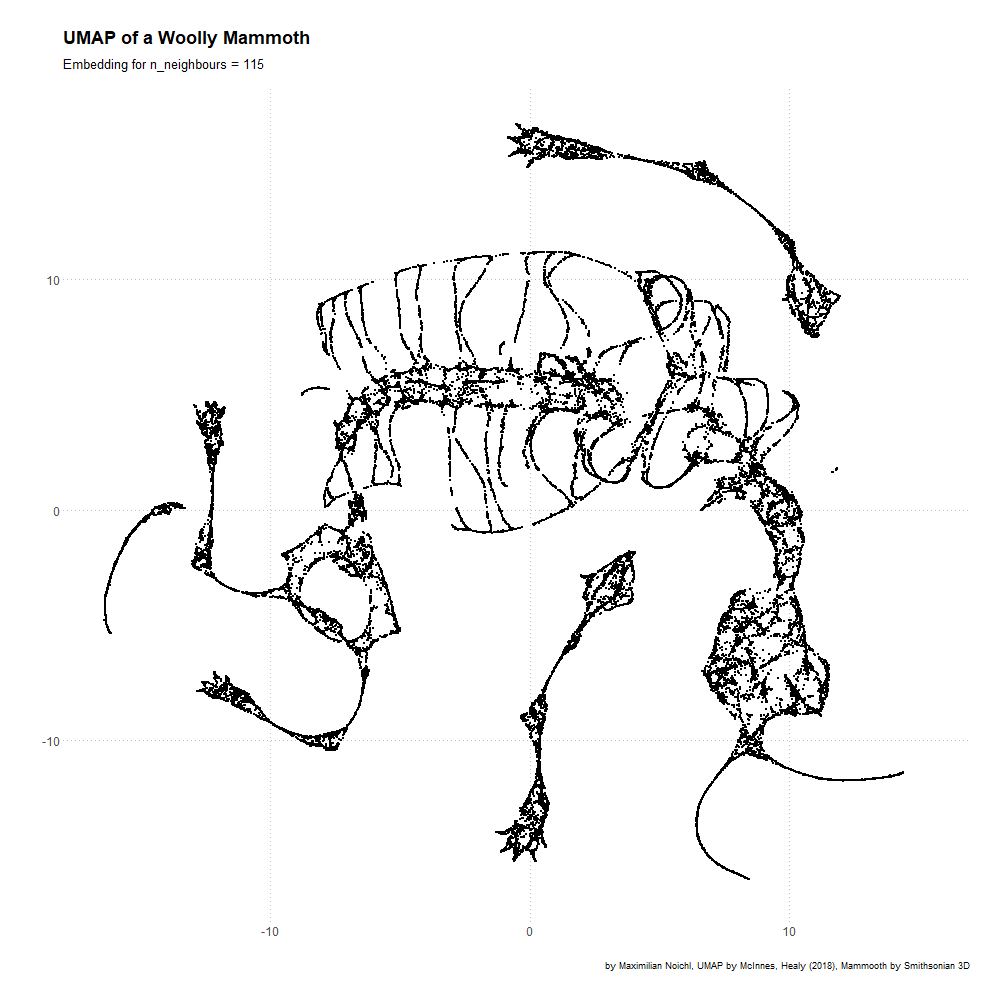
\includegraphics[width=\textwidth]{BERTopic/umap/n_neighbours115.png}
    \caption{$n\_neighbors = 115$}
\end{subfigure}
\caption{Proiezione UMAP di un modello 3D con 50\,000 punti in un piano 2D. Fonti: \href{https://3d.si.edu/object/3d/mammuthus-primigenius-blumbach:341c96cd-f967-4540-8ed1-d3fc56d31f12}{Smithsonian 3D Digitization Program} e \href{https://www.maxnoichl.eu/projects/mammoth/}{Max Noichl}.}
\label{fig:umap-mammoth}
\end{figure}
Si osservi come per valori ridotti di \texttt{n\_neighbors} la proiezione mantenga dettagli locali (curve delle zanne o delle zampe), ma perda la forma complessiva del mammut; all'aumentare del parametro la sagoma globale diventa riconoscibile, a scapito delle piccole variazioni geometriche. In modo analogo, sperimentare con valori come 15, 50 o 100 nel nostro dataset permette di calibrare il livello di granularità dei topic: valori molto bassi frammentano in gruppi minuti, mentre impostazioni alte tendono a fondere i cluster semantici più affini; una scelta intermedia (ad esempio \texttt{n\_neighbors} = 50) offre un equilibrio adeguato tra dettaglio locale e coerenza globale.
Per giungere a questa scelta sono stati provati diversi set di iperparametri; riportiamo di seguito quelli usati per la configurazione finale, così da facilitarne la riproducibilità:

\begin{lstlisting}[language=Python]
umap_model = UMAP(
    n_neighbors=n,
    n_components=10,
    min_dist=0.0,
    metric="cosine",
    random_state=1,
)
hdbscan_model = HDBSCAN(
    min_cluster_size=50,
    min_samples=15,
    metric="euclidean",
    cluster_selection_method="eom",
    prediction_data=True,
    cluster_selection_epsilon=0.1,
)
\end{lstlisting}

\begin{table}[H]
\centering
\footnotesize
\begin{tabular}{rrrrrr}
\hline
$n\_neighbors$ & $n\_topics$ & mean cluster size & std cluster size & topics $<100$ & topics $>500$ \\
\hline
15  & 15 & 208.87 & 267.01 & 8  & 2 \\
50  & 61 & 224.98 & 294.64 & 25 & 8 \\
60  & 62 & 197.81 & 254.00 & 26 & 6 \\
70  & 58 & 208.09 & 242.64 & 22 & 4 \\
100 & 2  & 2396.50 & 2090.91 & 0  & 2 \\
\hline
\end{tabular}
\caption{Sintesi degli esperimenti al variare di $n\_neighbors$: numero di topic trovati, dimensione media e deviazione standard dei cluster, oltre al conteggio dei topic piccoli ($<100$ documenti) e molto grandi ($>500$ documenti).}
\label{tab:n-neighbors-summary}
\end{table}

\noindent Nel corso dei test abbiamo variato \texttt{n\_neighbors} tra i valori 15, 50, 60 e 70 (con un confronto a 100 come baseline), scegliendo infine \texttt{n\_neighbors} = 50 come compromesso ottimale; la Tabella~\ref{tab:n-neighbors-summary} riassume il numero di topic e la distribuzione delle dimensioni dei cluster ottenuti in ciascun caso.

\begin{figure}[H]
\centering
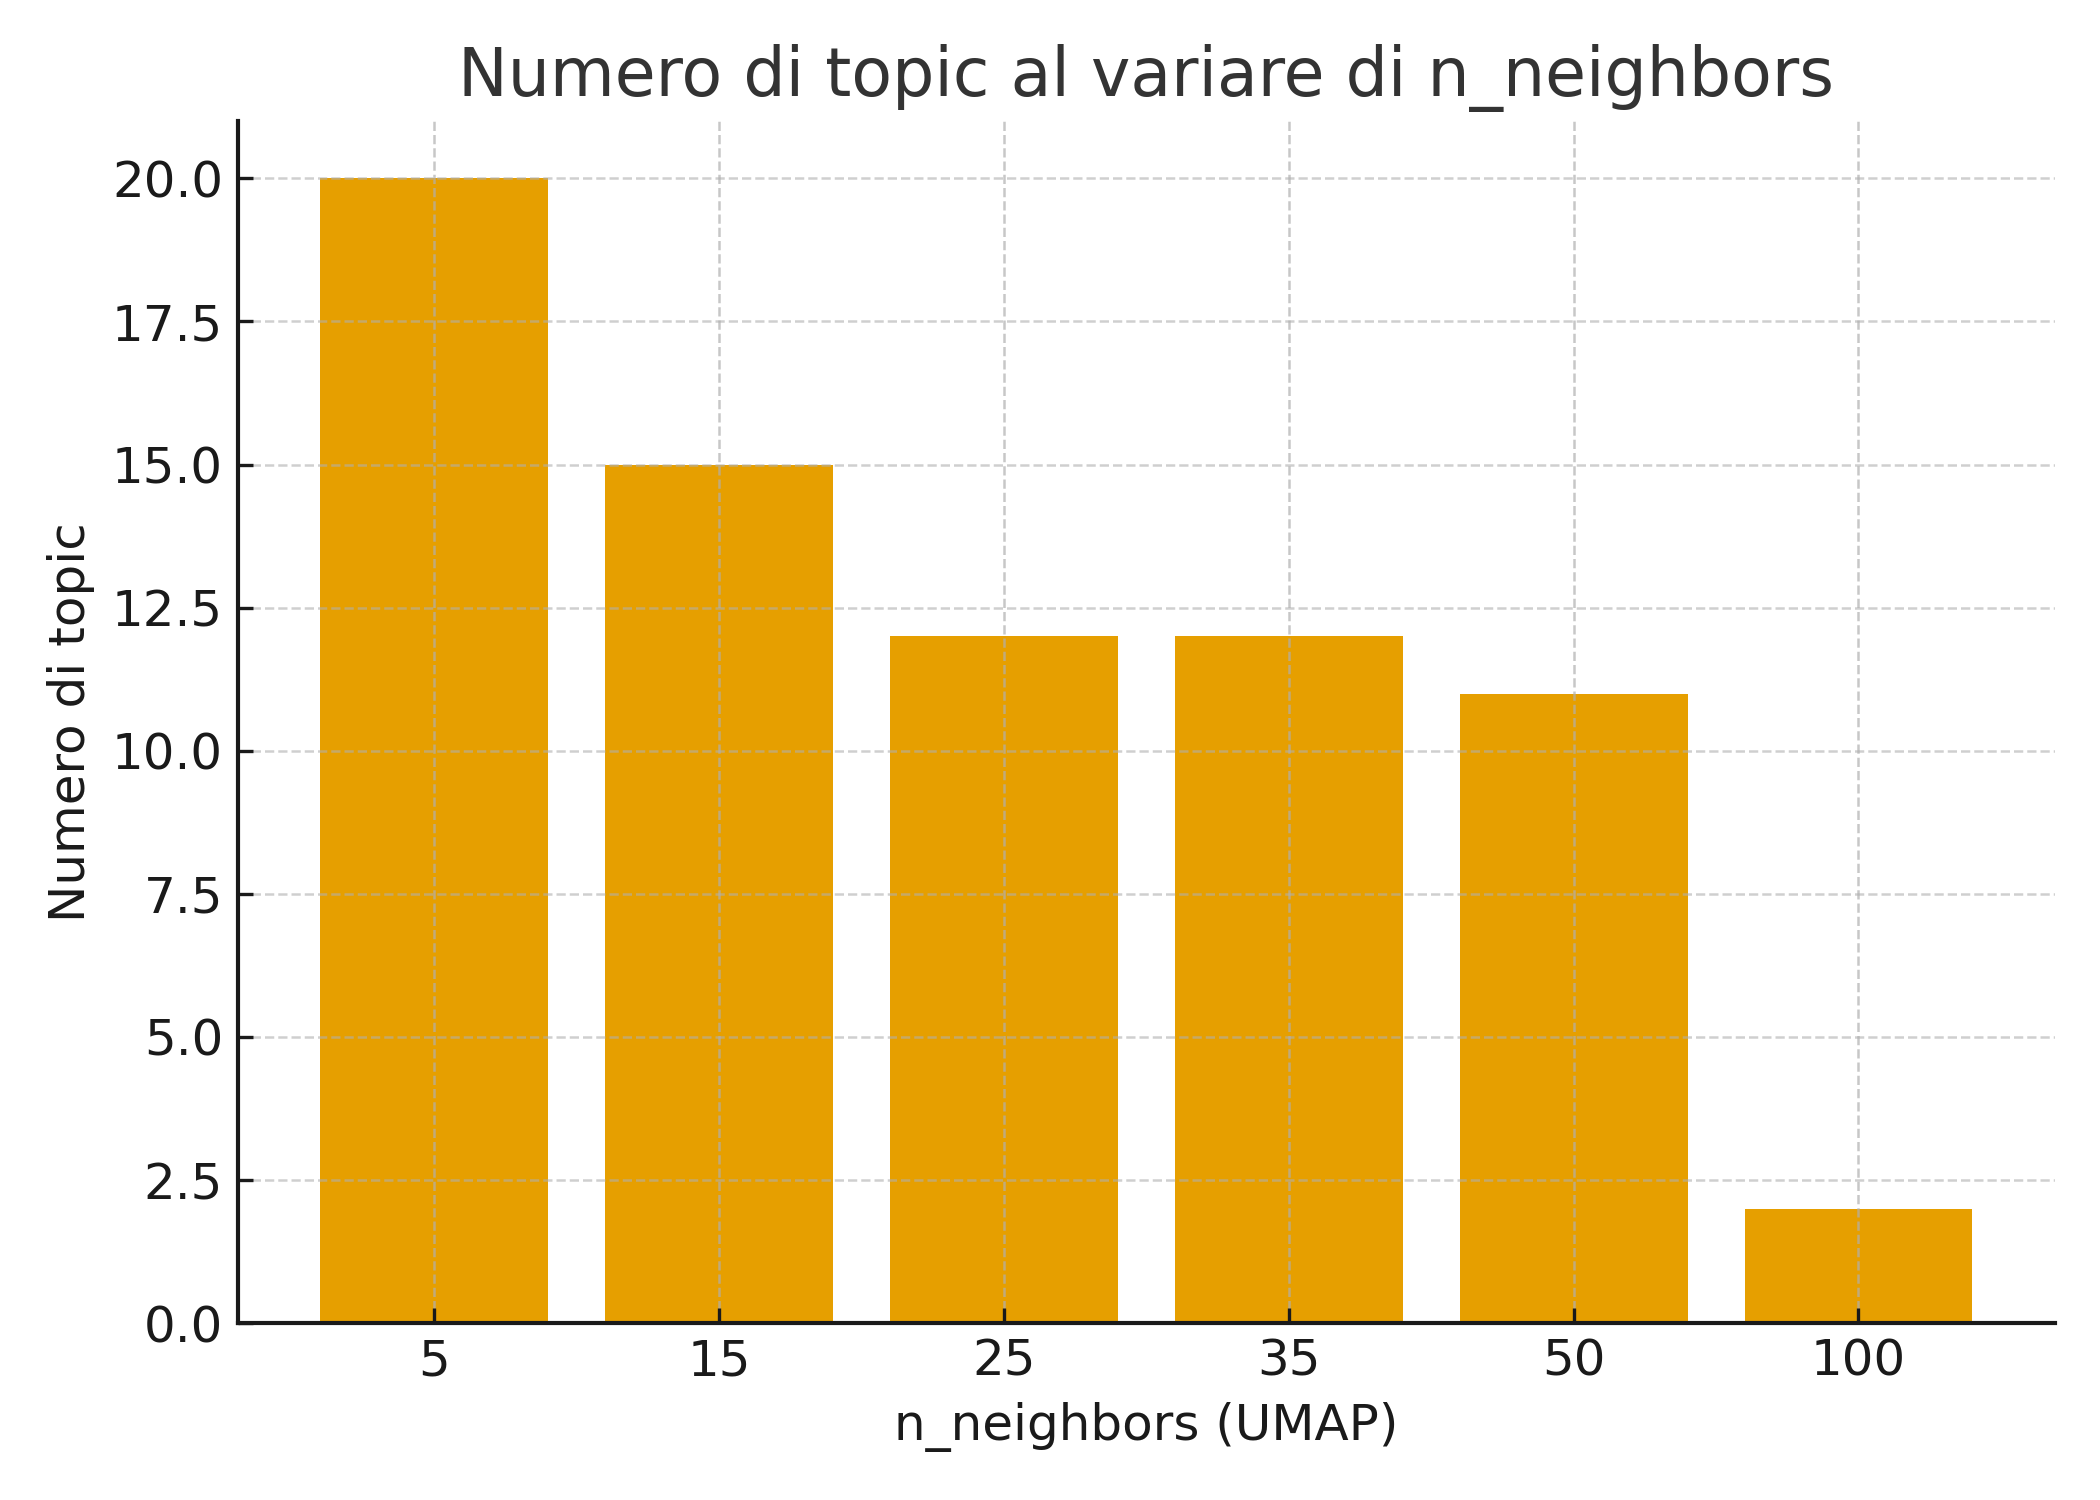
\includegraphics[width=0.6\textwidth]{BERTopic/umap/num_topics_per_neighbors.png}
\caption{Numero di topic generati da HDBSCAN al variare di $n\_neighbors$: la scelta intermedia ($n\_neighbors=50$) massimizza la granularità senza collassare in pochi cluster.}
\label{fig:num-topics-per-neighbors}
\end{figure}
\noindent I plot in Figura~\ref{fig:umap-neighbors-comparison} mostrano la proiezione bidimensionale generata da \texttt{BERTopic.\allowbreak visualize\_documents()} per tre configurazioni distinte. Con \texttt{n\_neighbors} = 15 UMAP costruisce un grafo molto \textbf{frammentato}: le connessioni tra i documenti sono deboli, molti punti rimangono isolati e HDBSCAN li etichetta come \textit{outlier}, generando quindi un topic \texttt{-1} (il topic dove vengono inseriti i documenti di cui si è incerti) estremamente popoloso (2224 documenti). All'estremo opposto (\texttt{n\_neighbors} = 100) il grafo è troppo \textbf{compatto}: le relazioni globali dominano e i topic tendono a fondersi. Con \texttt{n\_neighbors} = 50, invece, i cluster si addensano in regioni coerenti, evidenziando macro-categorie professionali distinte (marketing, cybersecurity, biomedical engineering, \emph{etc.}). L'incrocio tra indicatori numerici e analisi visiva conferma quindi \texttt{n\_neighbors} = 50 come valore finale.

\begin{figure}[H]
\centering
\begin{subfigure}{0.32\textwidth}
    \centering
    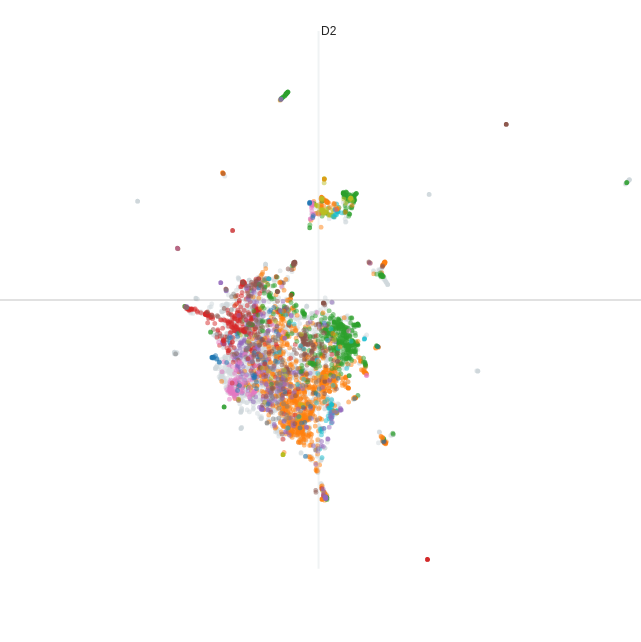
\includegraphics[width=\textwidth]{BERTopic/umap/umap_15.png}
    \caption{$n\_neighbors = 15$}
\end{subfigure}\hfill
\begin{subfigure}{0.32\textwidth}
    \centering
    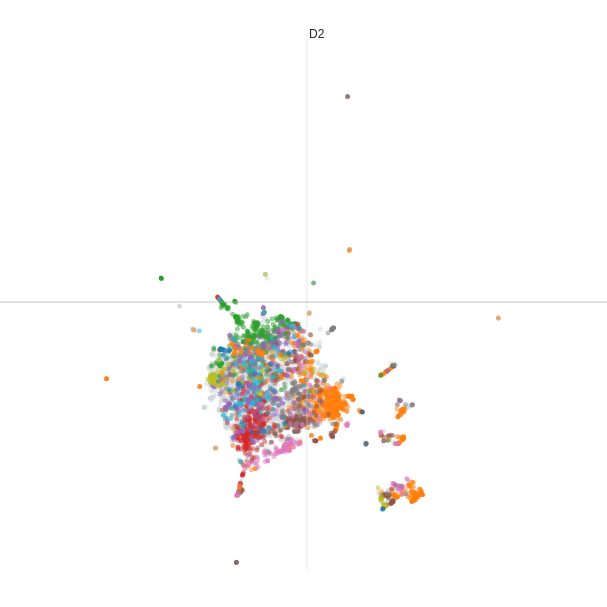
\includegraphics[width=\textwidth]{BERTopic/umap/umap_50.png}
    \caption{$n\_neighbors = 50$}
\end{subfigure}\hfill
\begin{subfigure}{0.32\textwidth}
    \centering
    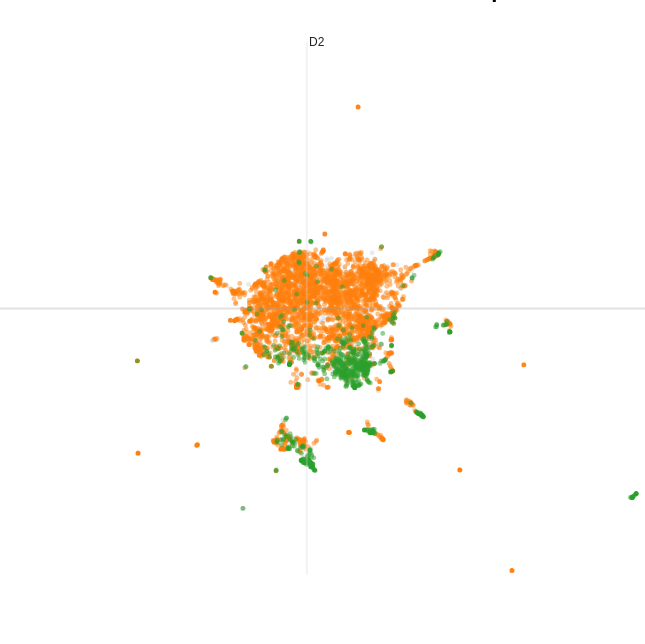
\includegraphics[width=\textwidth]{BERTopic/umap/umap_100.png}
    \caption{$n\_neighbors = 100$}
\end{subfigure}
\caption{Proiezioni generate da \texttt{BERTopic.\allowbreak visualize\_documents()}: i punti (embedding ridotti a 2 dimensioni) sono colorati in base al topic. Confronto tra \texttt{n\_neighbors} pari a 15, 50 e 100.}
\label{fig:umap-neighbors-comparison}
\end{figure}


\paragraph{\texttt{min\_dist}} controlla la densità minima consentita nella proiezione a bassa dimensione. Un valore vicino a zero permette ai punti di collassare in regioni molto dense, mettendo in risalto cluster ben separati; aumentando il parametro, UMAP distribuisce i punti con maggiore uniformità, sacrificando la compattezza dei gruppi a favore di una rappresentazione più omogenea. La Figura~\ref{fig:umap-min-dist} mostra come diverse configurazioni di \texttt{min\_dist} modifichino la distribuzione dei punti: valori estremamente bassi generano isole molto concentrate, mentre impostazioni più elevate distendono l'intero spazio proiettato.
\begin{figure}[H]
\centering

\begin{subfigure}{0.32\textwidth}
    \centering
    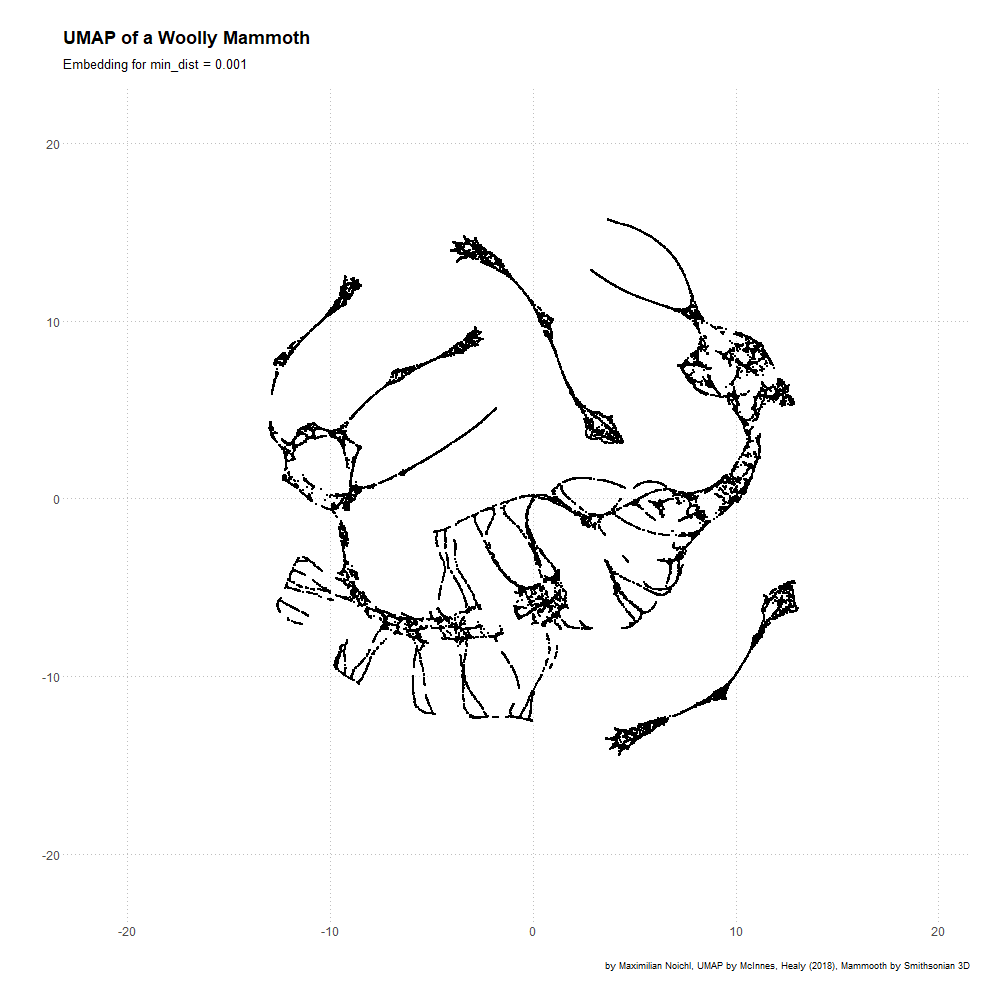
\includegraphics[width=\textwidth]{BERTopic/umap/min_dist_001.png}
    \caption{$min\_dist = 0.01$}
\end{subfigure}\hfill
\begin{subfigure}{0.32\textwidth}
    \centering
    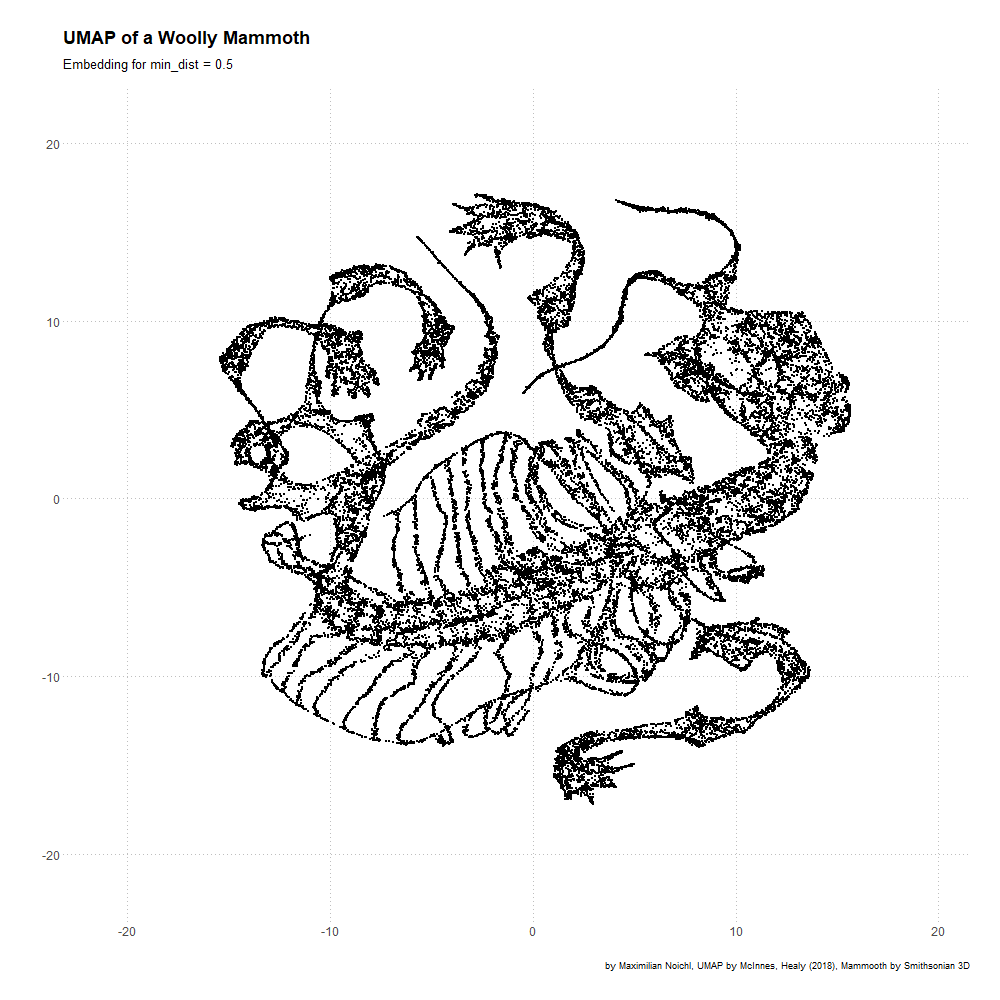
\includegraphics[width=\textwidth]{BERTopic/umap/m_dist_5.png}
    \caption{$min\_dist = 0.5$}
\end{subfigure}\hfill
\begin{subfigure}{0.32\textwidth}
    \centering
    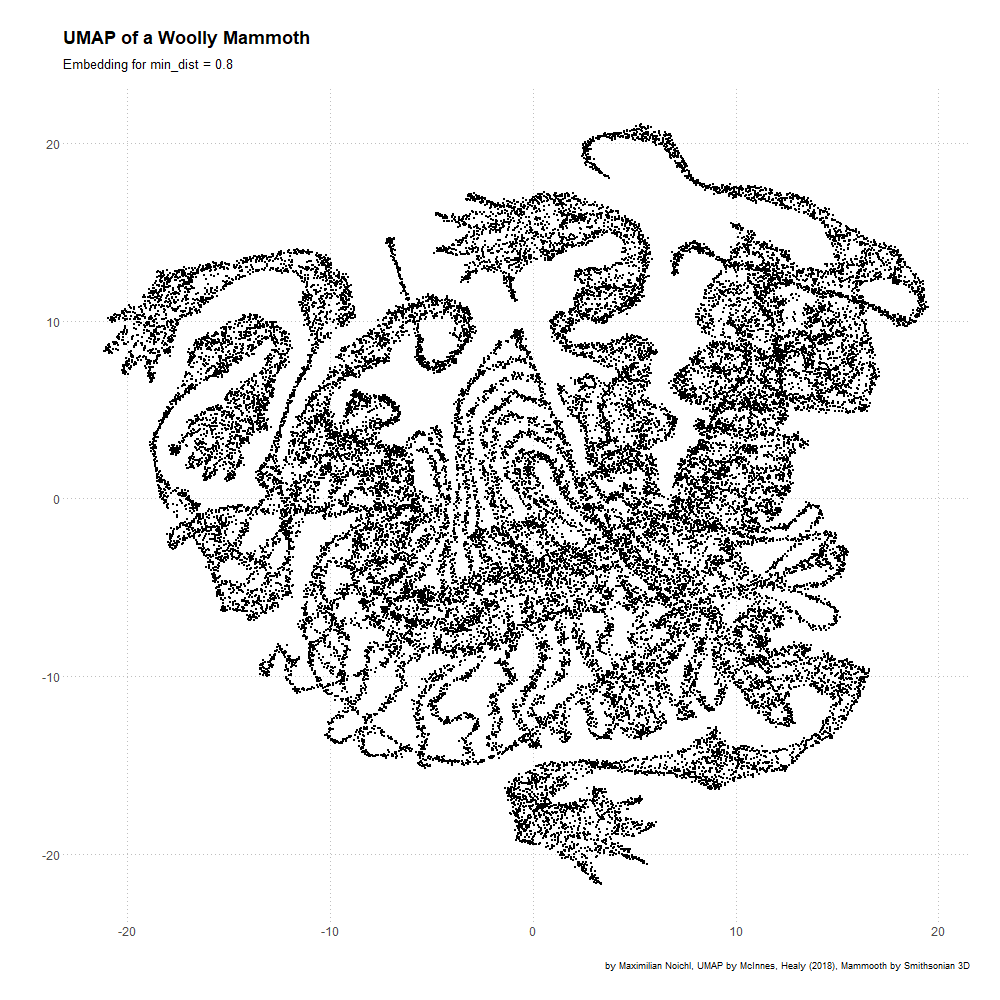
\includegraphics[width=\textwidth]{BERTopic/umap/m_dist_8.png}
    \caption{$min\_dist = 0.8$}
\end{subfigure}
\caption{Effetto di \texttt{min\_dist} sulla proiezione UMAP del modello 3D da 50\,000 punti. Fonti: \href{https://3d.si.edu/object/3d/mammuthus-primigenius-blumbach:341c96cd-f967-4540-8ed1-d3fc56d31f12}{Smithsonian 3D Digitization Program} e \href{https://www.maxnoichl.eu/projects/mammoth/}{Max Noichl}.}
\label{fig:umap-min-dist}
\end{figure}
\noindent Abbiamo fissato \texttt{min\_dist} a $0.0$ poiché l'algoritmo di \emph{clustering} (HDBSCAN) restituisce risultati migliori con cluster densi e ben separati: eventuali regioni vuote verrebbero classificate come outlier e assegnate al topic ``spazzatura'' (\texttt{-1}). Mantenere gli embedding compatti riduce la formazione di tali zone.

\subsection{Clustering}


\subsection{Tokenizer}
Dettagliare il tokenizer utilizzato, le strategie di pre-processing e qualsiasi personalizzazione per il dominio degli annunci di lavoro.

\subsection{Cosa si può migliorare}
Discutere criticità note, possibili ottimizzazioni della pipeline e idee per estensioni future di BERTopic nel progetto.
